\section{Results and Discussion}
System-level simulation was performed with representative AI inference workloads.

\subsection{Standby Power}
Migrating cold data and checkpoints to the FeRAM-backed tier yields more than 30\% reduction in standby power.
This reduction arises from suppressing periodic DRAM refresh for inactive regions.

\subsection{Resume Latency}
FeRAM allows direct restore of checkpoints without full DRAM wake-up.
Resume latency is reduced to the $\mu$s range, enabling near-instant resume after power gating and improving energy efficiency for mobile edge AI.

\subsection{Endurance}
FeRAM endurance of $10^{12}$~writes/year fits within FeRAM capability for checkpoint traffic.

% ===== Fig.2: Access time vs. retention (final) =====
\begin{figure}[!t]
\centering
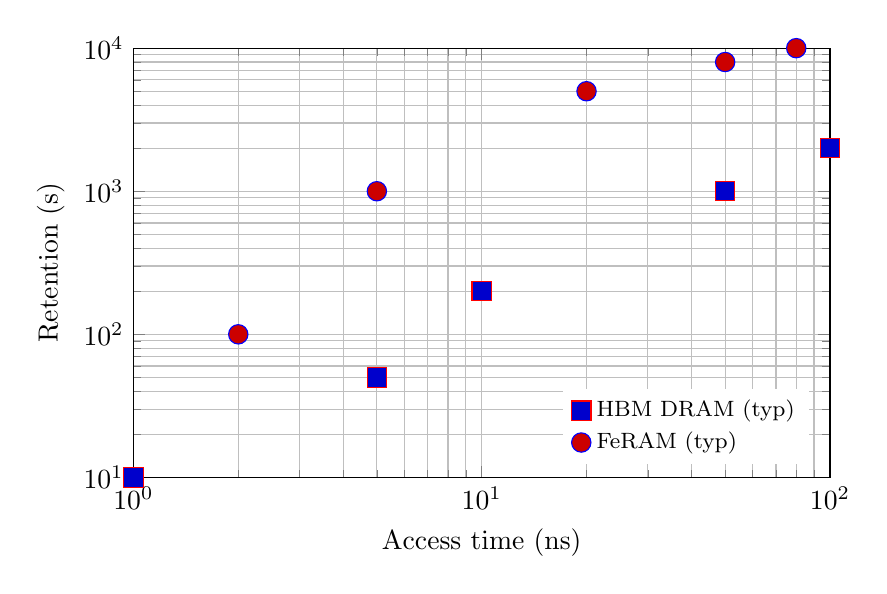
\begin{tikzpicture}
\begin{axis}[
  width=0.86\linewidth, height=0.58\linewidth,
  xmode=log, ymode=log,
  xmin=1, xmax=100, ymin=10, ymax=10000,
  xlabel={Access time (ns)}, ylabel={Retention (s)},
  grid=both, tick align=inside,
  legend style={draw=none, fill=white, font=\footnotesize},
  legend cell align=left, legend pos=south east
]
  % --- HBM: 赤い塗りつぶし四角(低い保持)---
  \addplot+[only marks, mark=square*, mark size=3.5pt, draw=red, fill=red]
    coordinates {(1,10) (5,50) (10,200) (50,1000) (100,2000)};
  \addlegendentry{HBM DRAM (typ)}

  % --- FeRAM: 青い塗りつぶし丸(高い保持)---
  \addplot+[only marks, mark=*, mark size=3.5pt, draw=blue, fill=blue]
    coordinates {(2,100) (5,1000) (20,5000) (50,8000) (80,10000)};
  \addlegendentry{FeRAM (typ)}
\end{axis}
\end{tikzpicture}
\caption{Access time vs. retention. HBM: red filled squares; FeRAM: blue filled circles.}
\label{fig:access_vs_retention}
\end{figure}
